\section{Results}
\label{sec:results}
Figure \ref{fig:grafGra} shows the knowledge graph generated by the query shown in listing \ref{lst:script5}. It is appreciated that the rectangles in purple contain the name of the object and those in fuchsia represent the identifier of the object. Each object can have zero or more relationships to other objects\footnote{Strictly speaking they only relate to objects that are part of the query.}. However, an object unrelated to others is of no use because it could not be reached since it has no edges, which represent ontological relationships. In addition, implicit or explicit information can be extracted through the edges (green lines).
% La Figura \ref{fig:grafGra} muestra el grafo de conocimiento generado por la consulta mostrada en listing \ref{lst:script5}. Se aprecia que los rectángulos en morado contienen el nombre del objeto y los de fiusha representan el identificador del objeto. Cada objeto puede tener cero o más relaciones con otros objetos\footnote{En estricto sentido solo se relacionan con objetos que son parte de la consulta.}. Sin embargo, un objeto sin relación con otros no es de utilidad debido a que no se podría llegar a él, puesto que no tiene aristas, las cuales representan las relaciones ontológicas. Además, a través de las aristas (líneas en verde) se puede extraer información implícita o explícita.

\lstinputlisting[language=Python, firstline=9, lastline=17,
caption=Query to generate the knowledge graph., label={lst:script5}]{code/queries.gql}
% caption=Consulta para generar un grafo de conocimiento,label={lst:script5}]{code/queries.gql}

\begin{figure}[H]
    \centering
    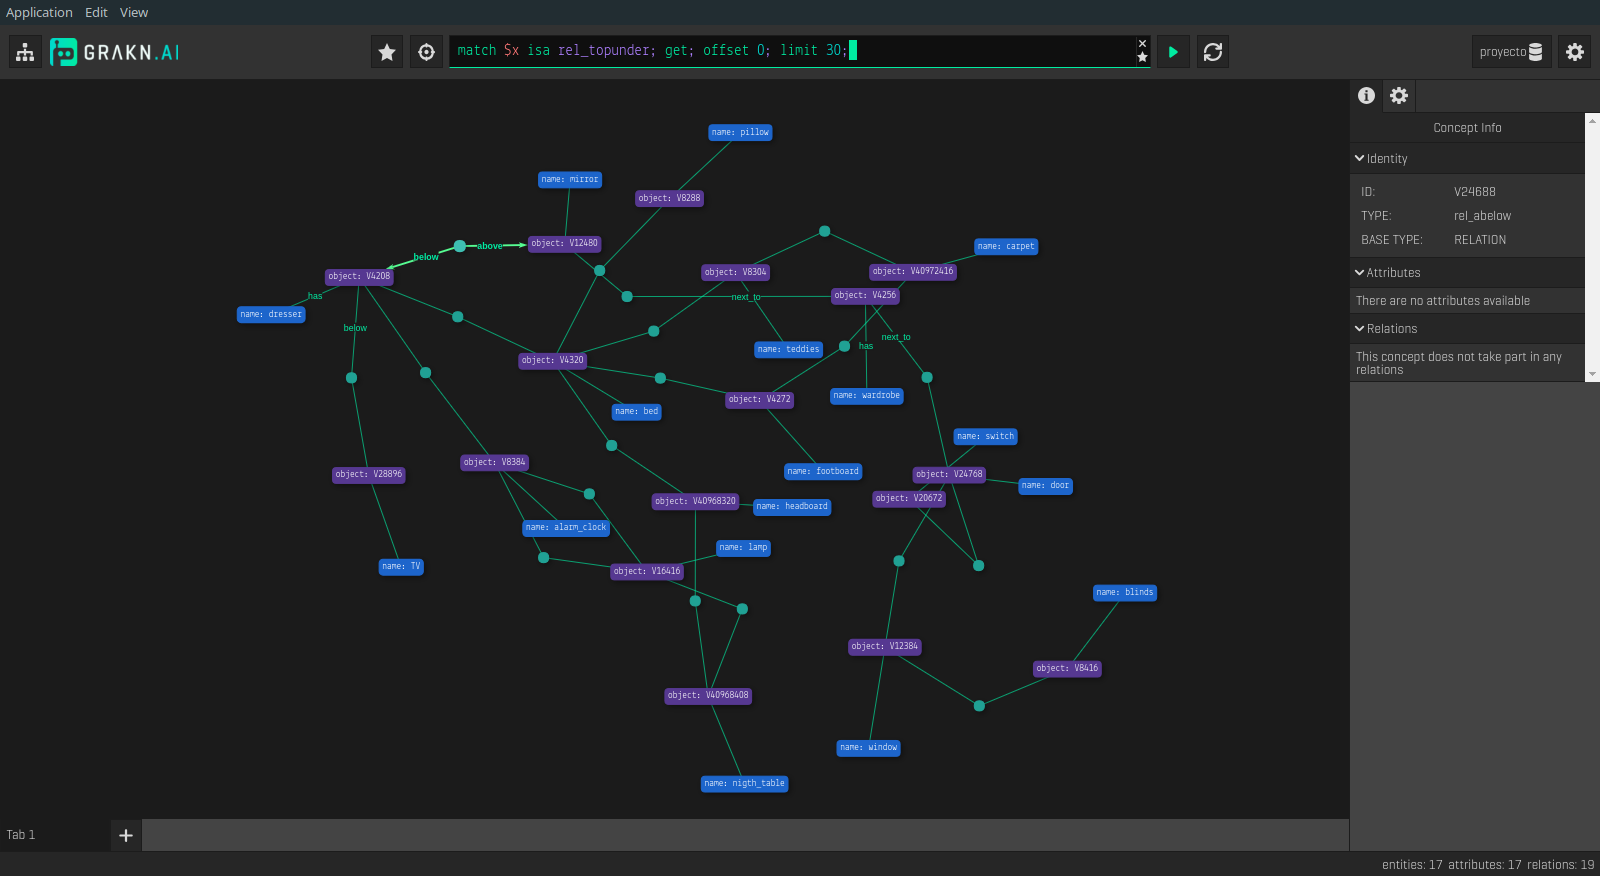
\includegraphics[width=8.8cm]{figures/allrel.png}
    \caption{Knowledge graph in Grakn.}
    % \caption{Grafo en Grakn}
    \label{fig:grafGra}
\end{figure}

The explicit information obtained from the edges explains why the objects were determined to be related. In most cases it is by the nature of the \textit{query} that it is executed. On the other hand, the implicit information is related to the \textit{background} of the relation of objects and is usually used when making inferences, better known as \textit{automatic reasoning}. It is worth mentioning that in this work we only work with explicit relationships.
% La información explícita que se obtiene de las aristas explica por qué se determinó relacionar los objetos. En la mayoría de los casos es por la naturaleza de la \textit{query} que se ejecuta. Por otra parte, la información implícita esta relaciona con el \textit{background} de la relación los objetos y se suele utilizar al realizar inferencias, mejor conocido como \textit{razonamiento automático}. Cabe mencionar que en este trabajo solo se trabaja con relaciones explícitas.

Figure \ref{fig:ReGra} shows the relationship \textit{rel-topunder} between the bed and footboard which can be expected while finding the object ``footboard'' under the object ``bed'' and the object ``bed'' in top of the ``footboard''. Also, in the same image, the \textit{rel-abelow} relationship between footboard and carpet can be seen similarly to the previous one.
% La Figura \ref{fig:ReGra} muestra la relación \textit{rel-topunder} entre la cama y el pie de cama (bed-footboard), lo que indica que se espera encontrar al objeto ''pie de cama'' debajo del objeto ''bed'' y al objeto ''bed'' sobre el ''footboard''. Asimismo, en la misma imagen se aprecia de manera similar a la anterior la relación \textit{rel-abelow} entre footboard y carpet.

\begin{figure}[H]
    \centering
    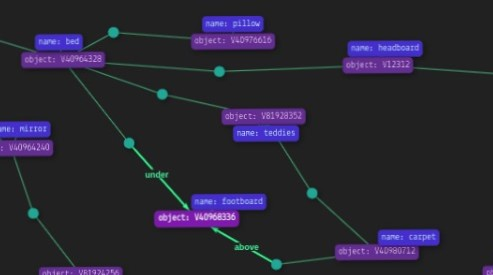
\includegraphics[width=8.4cm]{figures/realcionGrafo.jpeg}
    \caption{Relation bed-footboard, footboard-carpet.}
    % \caption{Relación bed-footboard, footboard-carpet}
    \label{fig:ReGra}
\end{figure}

%% NEW 
% a) uno al final en la sección de resultados, después de la Fig. 12, en el que se clarifique el por qué fue necesario hacer este estudio de KG para la caracterización de objetos de un determinado espacio interior de ocupación humana, como es una habitación de una vivienda.

This work is a contribution to the categorization of the semantic context in computer vision since it establishes the tools and a baseline in spatial relationships to create maps of the environment of places of human occupation, using knowledge graphs, in contrast to the common way it is usually done.

Normally, to avoid processing an immense quantity of convolutions, which translates into higher execution time, \cite{Galleguillos} suggests creating object context base on object scale or spatial context, by creating big comparison lists (dataset) and contrasting them with image training sets. This is a good approach, however, the list remains static and does not get feedback from the training dataset. Which our model does naturally because that is how knowledge graphs work.